%!TEX root = ../thesis.tex

\section{Local Deployment}
\label{sec:local_infrastructure}

The local deployments consists of the residential communication gateway and the deployed digital thermostats with their wireless adapters.
The communication gateway collects the data read from the thermostats and sends it to the remote web server.
The digital thermostats are programmable and allow us to modify their behavior by flashing custom firmware.
This project uses the work of a previous master thesis as a basis to build upon\cite{eigenmann2012opportunisticSensing}.
The primary focus is to improve the basic functionality of the communication gateway and create an unified but loosely coupled infrastructure by using the RESTful API provided by the server.
See also Figure~\ref{fig:residence_layout} for an overview of the local deployment.

\begin{figure}[h]
	\begin{center}
		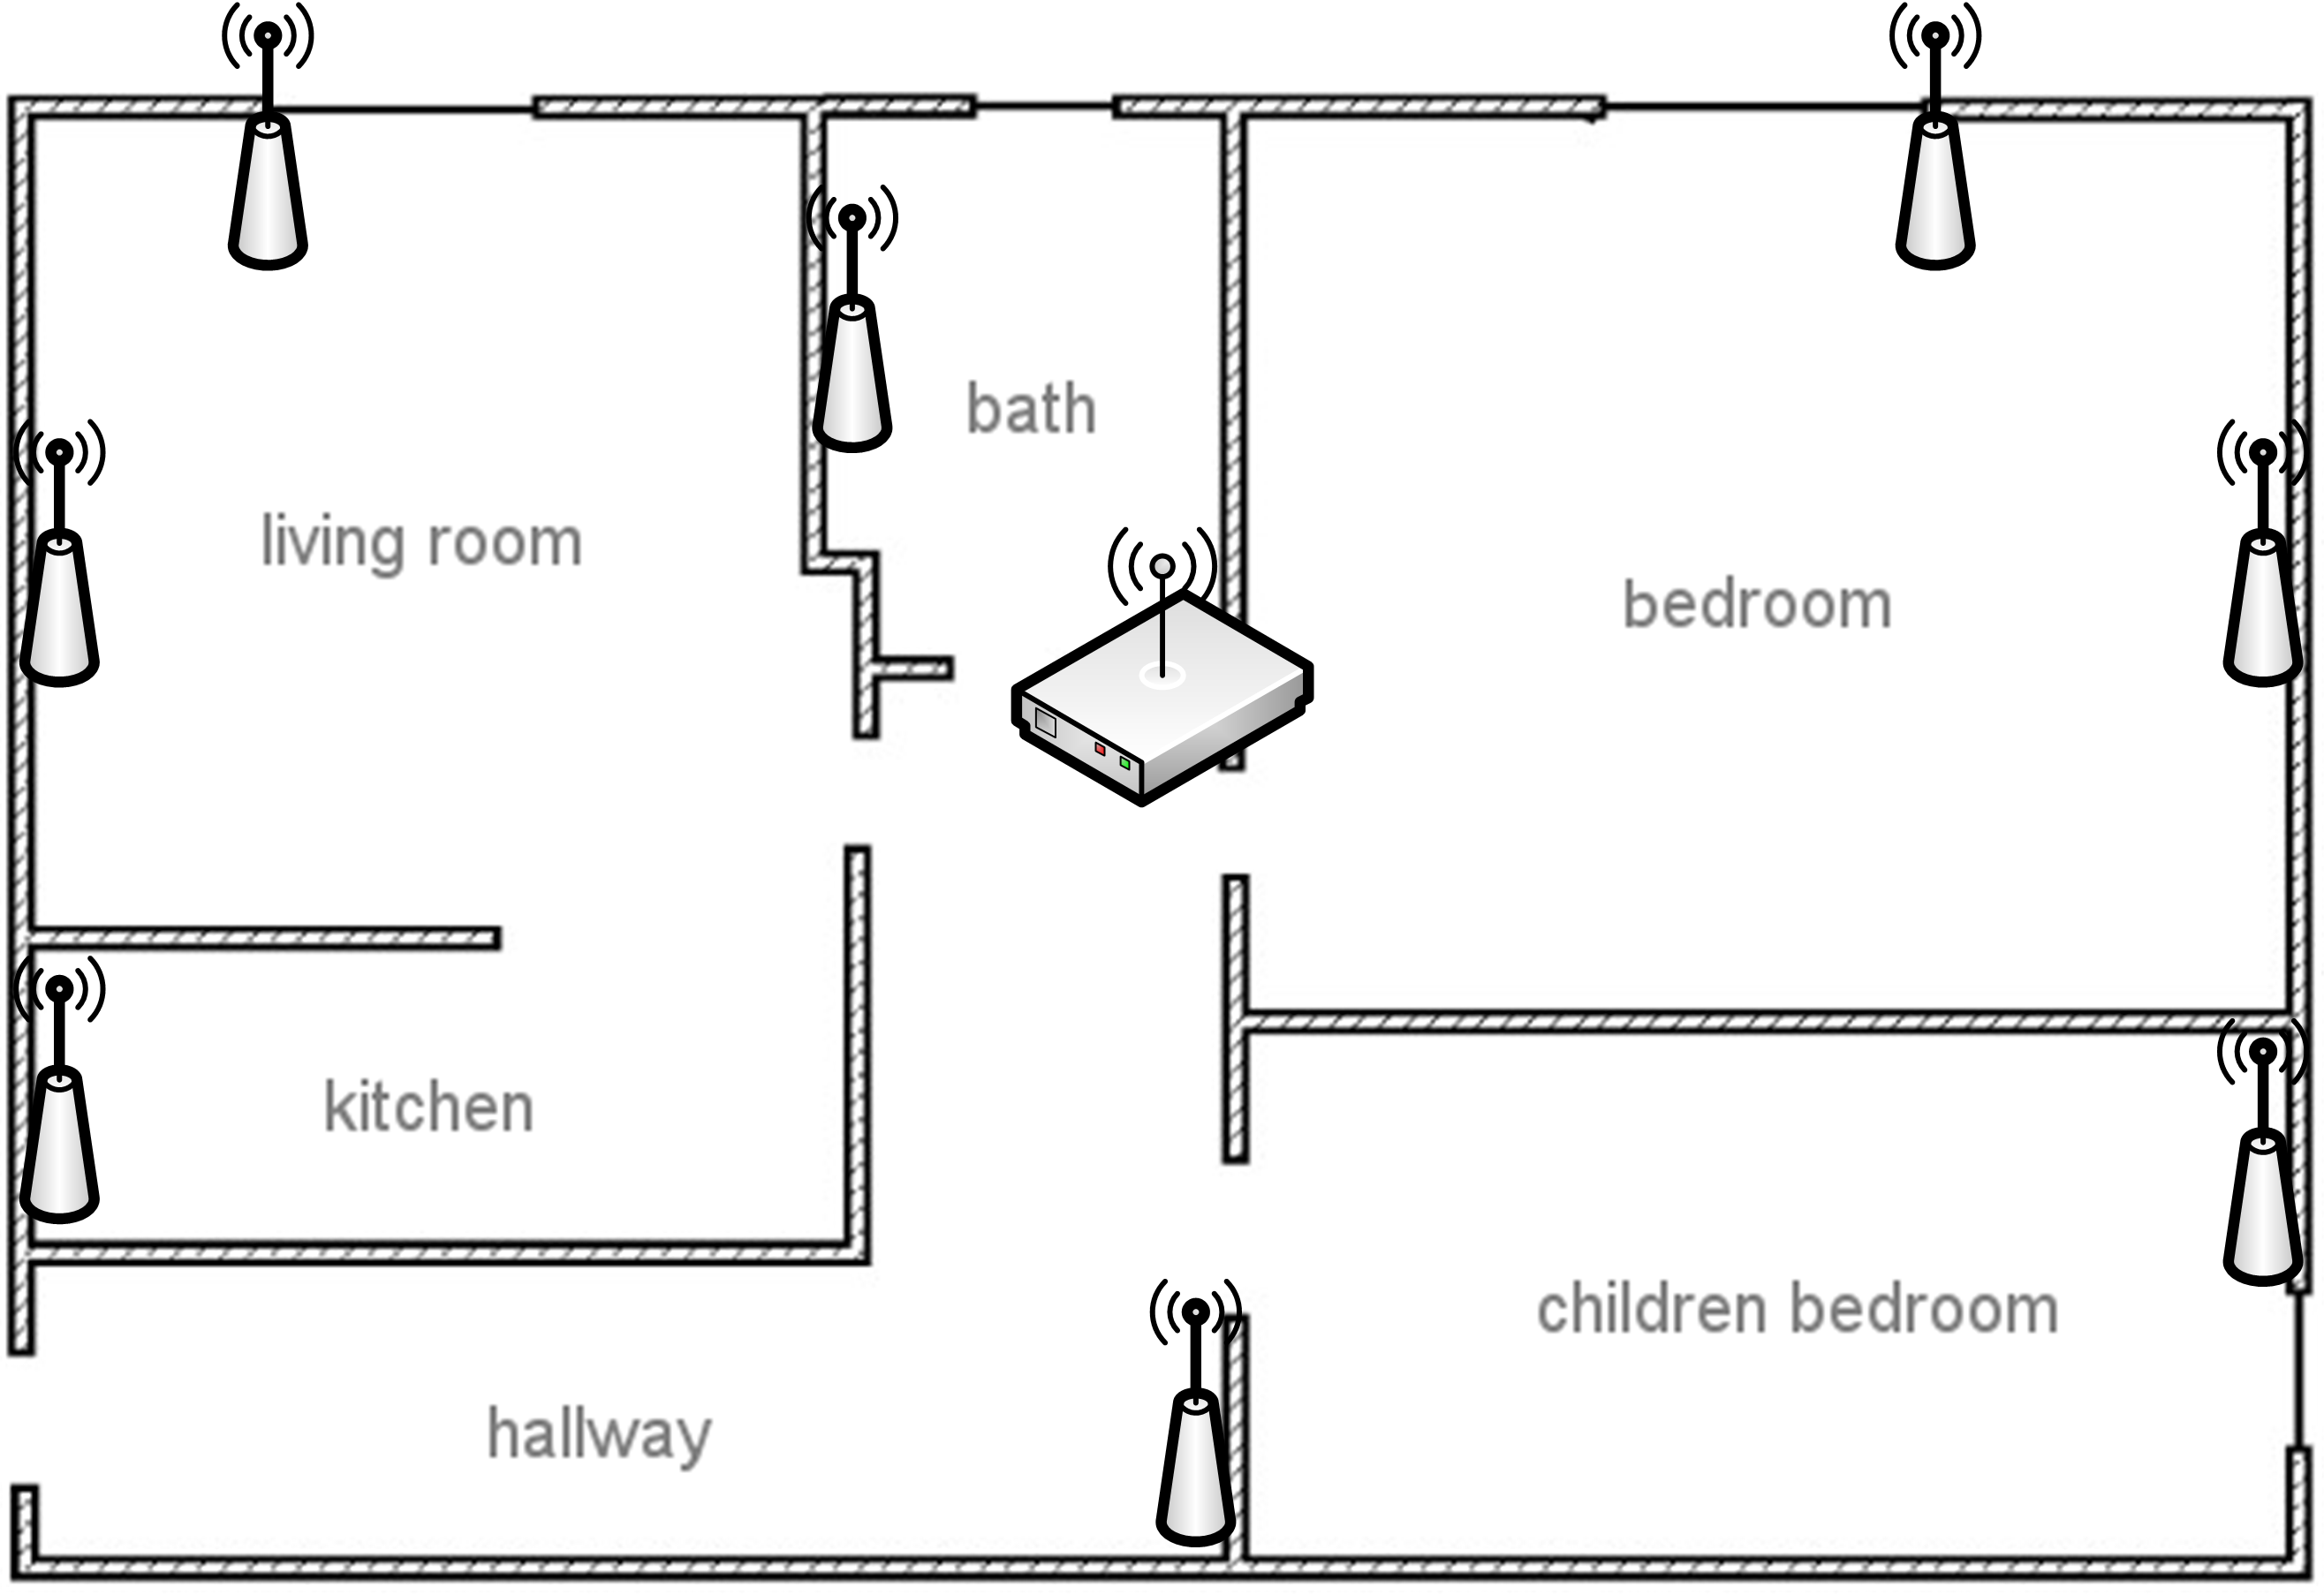
\includegraphics[width=0.7\textwidth]{images/residence_layout_schema.png}
	\end{center}
	\caption{Example of a residence layout depicting a possible deployment. The local communication gateway is installed in the hallway, connected to the internet and has wireless connections to the deployed thermostats represented as antennas. Source of the original image: \url{http://www.haus-topplicht.de/wp-content/uploads/2013/12/planwohnung2.jpg}}
	\label{fig:residence_layout}
\end{figure}

\subsection{Existing Infrastructure}

This project builds upon work previously done by Nico Eigenmann as his master thesis \cite{eigenmann2012opportunisticSensing}.
Part of his work consisted of extending the hardware and software of the digital thermostat HR-20\footnote{\url{http://www.homexpertbyhoneywell.com/en-DE/Products/rondostat/Pages/HR-20.aspx}}, as depicted in Figure~\ref{fig:honeywell_hr20}, to offer wireless access via 6LoWPAN\footnote{6LoWPAN is an acronym of IPv6 over Low power Wireless Personal Area Network}.
Further a border router translates the 6LoWPAN messages into IPv6 packets and vice versa.
This border router is connected per Universal Serial Bus (USB) port to a computer and communicates via Serial Line Internet Protocol (SLIP).
The computer redirects the received packets into the connected Local Area Network (LAN) and also routes messages addressed to a sensor in the 6LoWPAN network via the border router.

\begin{figure}[h]
%\begin{wrapfigure}{r}{0.45\textwidth}
	\begin{center}
		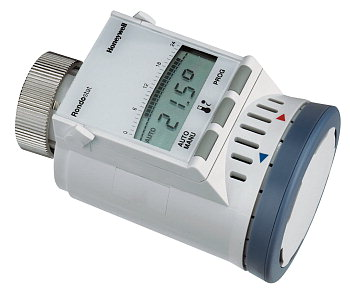
\includegraphics[width=0.4\textwidth]{images/hr20.jpg}
	\end{center}
	\caption{Honeywell Rondostat HR-20 programmable thermostat. Source: \url{https://piontecsmumble.files.wordpress.com/2013/02/hr20.jpg}}
	\label{fig:honeywell_hr20}
\end{figure}

\subsection{Design Goals}

Several design goals are determined in order to evaluate the system design and implementation.

\begin{itemize}
	\item \emph{Performance} for low computational effort and power consumption on embedded systems.
	\item \emph{Reliability} for a high probability that the system operates as expected.
	\item \emph{Robustness} to let the system behave reasonably in presence of failures, especially connection problems.
	\item \emph{Interoperability} to cooperate with other distributed systems.
\end{itemize}

\subsection{Software Platform and Frameworks}

This sub section lists and describes the software components used on the local communication gateway.

\paragraph{tunslip6} is a tool to route IPv6 packets between the host and a border router via serial line.
It is used to create a tunnel interface an the host system which acts as a regular network interface.

\paragraph{Python} is a multi-paradigm programming language and is suitable for desktop as well as for embedded systems.
This allows us to use a single programming language for the implemented software parts in the whole infrastructure on the local and server side.
Further Python includes packages to facilitate asynchronous input and output which is required to concurrently query multiple network resources.

\paragraph{Constrained Application Protocol (CoAP)} \cite{rfc7252} is a application protocol created for low power devices and sensors that are heavily restricted in terms of computing power, memory size and power consumption.
Unlike the Hypertext Transfer Protocol (HTTP) commonly used in desktop and mobile systems, CoAP is based on minimalistic network protocols to reduce overhead and computational requirements.

\paragraph{aiocoap} is a third-party package for Python implementing the CoAP protocol.

\paragraph{requests} is a library written in Python providing a simple and well designed interface to send HTTP requests.
This is used to communicate with the API provided by the Smart Heating Server.

\subsection{Implementation}
\label{sec:local_infrastructure_implementation}

The implementation work on the local infrastructure focuses on the local computer acting as a local communication gateway, this two terms are further used interchangeably.
We use the Raspberry Pi 2 Model B\footnote{\url{https://www.raspberrypi.org/products/raspberry-pi-2-model-b/}} as our local communication gateway which is responsible for two major tasks.

First, it needs to periodically query the temperatures and other meta data from the digital thermostats and store the data locally.
Additionally the heating scheduling algorithm determines the current target temperature and applies the value to the thermostats.
Second, the local computer consistently synchronizes the local data storage with the remote Smart Heating Server.
The new data gathered from the thermostats is therefore sent to the server and the latest configuration such as the heating schedule is downloaded.

The local computer works as a proxy server and enables the local deployment to operate independently from the connection to the remote server.
This way the last downloaded heating schedule is kept and operated until the server connection is reestablished.

% TODO?
%\todo[inline]{Overview picture of the used local deployment: thermostat, radio module powerd by USB, Raspbeery with border router\\
%	Honeywell HR-20, Radio Module deRFmega128, USB powered}

All the code, binaries and instructions required to setup the Raspberry Pi 2 are provided in the Git repository located at \url{https://github.com/spiegelm/smart-heating-local}.
We highly encourage the reader to visit the project on GitHub.
The repository is designed to be self contained.
This means in order to setup a local communication gateway only the hardware, a copy of the repository and an internet connection are needed.
A step-by-step instruction to setup the software on a Raspberry Pi 2 is included in the \highlight{README.md} file.

\subsubsection{Border Router Connection}

Upon connection of the border router at an USB port the corresponding rule in \highlight{/etc/udev/rules.d/90-local.rules} is executed.
The rule executes the file \highlight{bin/start\_tunslip.sh} in the code repository to establish a tunnel to the border router using tunslip6.
The border router runs a web server providing information about connected thermostat devices.
The log file \highlight{/var/log/tunslip6} generated by tunslip6 shows the associated web server address:

\begin{lstlisting}[numbers=none, moredelim={[is][keywordstyle]{@@}{@@}}]
Server IPv6 addresses:
 @@fdfd::212:7400:115e:a9e5@@
 fe80::212:7400:115e:a9e5
\end{lstlisting}

The address with the prefix \highlight{fdfd:} is the one we want. Requesting the determined URI \nolinkurl{http://[fdfd::212:7400:115e:a9e5]} returns an HTML table containing all discovered devices:
%, as shown in Listing~\ref{lst:border_router_devices}.

%\begin{lstlisting}[label={lst:border_router_devices}, caption={Example of routing table provided by the border routers web service}]
\noindent
\begin{minipage}{\linewidth}
\begin{lstlisting}[numbers=none]
<html><head><title>ContikiRPL</title></head><body>
Neighbors<pre>fe80::221:2eff:ff00:228b</pre>
Routes<pre>fdfd::221:2eff:ff00:228b/128 (via fe80::221:2eff:ff00:228b) 16710893s</pre>
</body></html>
\end{lstlisting}
\end{minipage}

Each route corresponds to a CoAP URI. For example the URI \nolinkurl{coap://[fdfd::221:2eff:ff00:228b/128]/sensors/temperature} could be queried by a CoAP client to determine the currently measured temperature.

Please note: The discovered devices are not necessarily thermostats registered to the local communication gateway.
The linked thermostats are therefore retrieved from the Smart Heating Server to avoid unnecessary querying of unrelated devices.


\subsubsection{Executable Scripts}
\label{sec:local_infrastructure_implementation_scripts}

The \highlight{smart-heating-local} repository contains two python scripts in the repository root: \highlight{thermostat\_sync.py} and \highlight{server\_sync.py}.
Each script corresponds to one of the two tasks described in Section~\ref{sec:local_infrastructure_implementation}.
The first scripts is responsible for fetching the temperature and other measurements from the thermostats to the local storage and applying the latest heating schedule.
The latter script sends the measurements that where not yet delivered to the server and retrieves the most actual heating schedule. Both scripts are independent from each other and use only the local storage to share data as explained in Section~\ref{sec:local_infrastructure_implementation_storage} below.

\paragraph{Scheduling}

The periodic execution of the both scripts is scheduled by the \emph{cron} service which is provided by the deployed operating system \emph{Raspbian} and also by most Linux operating systems.
The \highlight{crontab} program is used for defining the schedule.

\subsubsection{Local Storage}
\label{sec:local_infrastructure_implementation_storage}

We combine SQLite and dbm for the local storage.
\emph{SQLite} is a lightweight relational database engine implementing most of the SQL standard and is often used on embedded systems.
\emph{dbm} is a family of simple database engines allowing to store pairs of a unique key and a value.
The two databases are used for different purposes.
The SQLite database persists historic measurement entries that should be held at least until they are transferred to the server.
On the other side there is the dbm database holding configurations retrieved from the server.
For example the thermostats associated with a local communication gateway and the current heating schedule are stored using dbm as it has no relational schema and is therefore much simpler to use and maintain.
Both databases are stored in files within the \highlight{data/} directory.

\subsubsection{Application}

All Python files containing application logic are located in the directory \highlight{smart\_heating\allowbreak \_local}.
%The directory is also a Python namespace.
The following paragraphs list the files within this directory and describe their purpose.

% TODO
%\todo[inline]{Cleanup the server files.}

\paragraph{config.py} contains the \highlight{Config} class responsible for storing and retrieving the heating schedule as also the thermostat MAC addresses linked to this Raspberry Pi computer.
The configuration is stored using the \highlight{shelve} Python package which itself builds on the npm database engine installed on the system.

\paragraph{server.py} provides an interface to communicate with the Smart Heating Server.
It also determines the URI schema used by the server API.

\paragraph{server\_models.py} contains the models used by the server.
The models correspond to the resources provided the server API and structure them into classes.

\paragraph{server\_controller.py} provides a layer of abstraction by packaging the most important functionality regarding server communication.
It makes use of the files \highlight{server.py} and \highlight{server\_models.py}.
The provided methods include downloading the latest heating schedule and the thermostat configuration linked to this local communication gateway as well as storing the data in the local storage using the \highlight{Config} class.

\paragraph{local\_models.py} contains the models handling the temperature measurements and meta data entries which are stored in the local database.

\paragraph{thermostat\_controller.py} is responsible for querying the thermostats defined in the configuration and saving the data into the SQLite database.
The controller also contains the logic regarding CoAP requests and the resource schema used by the digital thermostats.

\paragraph{tests/} is the directory containing the tests that were created during implementation and which assisted the application development.
The tests can be started using the command \highlight{nosetests -a '!local'} from the repository root.
These tests are also periodically executed and logged by the Continuous Integration service Travis CI\footnote{\url{https://travis-ci.org/}}.

\paragraph{logging/} contains the central logging configuration used in the whole local project.
Relevant information is logged to the file \highlight{logs/smart\_heating.log}.






